\documentclass[12pt]{article}

% Preamble and title page follow the TU-Sofia thesis template (Bulgarian layout,
% same faculty heading and typography).

\usepackage{cmap}
\usepackage[T2A]{fontenc}
\usepackage[utf8]{inputenc}
\usepackage[bulgarian]{babel}

% --- Typography ---
\usepackage{tempora}
\usepackage[top=2.5cm, bottom=2.5cm, left=3.0cm, right=2.0cm, a4paper]{geometry}
\usepackage{setspace}
\setstretch{1.5}
\usepackage[none]{hyphenat}
\usepackage[expansion=false]{microtype}
\emergencystretch=1.5em
\sloppy
\usepackage{indentfirst}
\setlength{\parindent}{1.25cm}
\setlength{\parskip}{0pt}

% --- Page numbering (bottom right) ---
\usepackage{fancyhdr}
\pagestyle{fancy}
\fancyhf{}
\renewcommand{\headrulewidth}{0pt}
\fancyfoot[R]{\thepage}

% --- Footnotes ---
\usepackage[hang,flushmargin]{footmisc}
\usepackage{ragged2e}
\renewcommand{\footnotelayout}{\fontsize{10}{12}\selectfont\setstretch{1.0}\justifying}

% --- Sections ---
\usepackage{titlesec}
\renewcommand{\thesection}{\Roman{section}}
\renewcommand{\thesubsection}{\arabic{section}.\arabic{subsection}}

\titleformat{\section}[block]
  {\fontsize{14}{16.8}\bfseries\centering}
  {\thesection. }
  {0pt}
  {\MakeUppercase}

\titleformat{\subsection}[block]
  {\fontsize{14}{16.8}\bfseries}
  {\thesubsection. }
  {0pt}
  {}
\titlespacing*{\subsection}{1.25cm}{*3}{*2}

% --- Table of contents ---
\usepackage{etoolbox}
\makeatletter
\patchcmd{\l@section}{#1}{\MakeUppercase{#1}}{}{}
\makeatother
\usepackage[titles]{tocloft}
\renewcommand{\cftsecleader}{\cftdotfill{\cftdotsep}}
\renewcommand{\cftsubsecleader}{\cftdotfill{\cftdotsep}}
\renewcommand{\cftsecfont}{\fontsize{12}{14}\bfseries}
\renewcommand{\cftsecpagefont}{\fontsize{12}{14}\bfseries}
\renewcommand{\cftsecaftersnum}{.}
\renewcommand{\cftsubsecaftersnum}{.}
\setlength{\cftsubsecnumwidth}{3em}
\setlength{\cftsecnumwidth}{3em}

% --- Captions ---
\usepackage{caption}
\addto\captionsbulgarian{\renewcommand{\figurename}{Фигура}}
\DeclareCaptionLabelFormat{tablelabel}{Таблица #2}
\captionsetup[table]{
    labelformat=tablelabel,
    labelsep=period,
    font={bf,small},
    justification=centering,
    singlelinecheck=true
}

% --- Other ---
\usepackage{amsmath}
\usepackage{graphicx}
\usepackage{longtable}
\usepackage{needspace}
\usepackage{listings}
\lstset{basicstyle=\ttfamily\footnotesize,breaklines=true,columns=fullflexible,keepspaces=true,frame=single}
\usepackage{float}
\usepackage{booktabs}
\usepackage{array}
\usepackage[hidelinks]{hyperref}

\AtBeginEnvironment{lstlisting}{\setstretch{1}}
\begin{document}
\hypersetup{pageanchor=false}
\begin{titlepage}
\begin{center}
{\fontsize{18}{21.6}\selectfont\bfseries ТЕХНИЧЕСКИ УНИВЕРСИТЕТ -- СОФИЯ\par}
\vspace{0.5cm}
{\fontsize{16}{19.2}\selectfont\bfseries ФАКУЛТЕТ „КОМПЮТЪРНИ СИСТЕМИ И ТЕХНОЛОГИИ“\par}
\vspace{0.6cm}

\includegraphics[width=0.28\linewidth]{images/tu_logo.png}
\vspace{0.8cm}

{\fontsize{20}{24}\selectfont\bfseries КОНФИГУРИРАНЕ И ДИАГНОСТИКА НА GRE ТУНЕЛ\par}
\vspace{0.8cm}
{\fontsize{14}{16.8}\selectfont\bfseries ЛАБОРАТОРЕН ПРОТОКОЛ\par}
\vspace{0.3cm}
{\fontsize{13}{15.6}\selectfont Упражнение 2\par Cisco Packet Tracer\par}
\vfill
\begin{flushleft}
{\fontsize{14}{16.8}\selectfont\bfseries Изготвил:\par}
Алекс Цветанов\par
Факултетен № 371326005\par
\vspace{0.5cm}
{\fontsize{14}{16.8}\selectfont\bfseries Преподавател:\par}
д-р Йонка Ганчева\par
\end{flushleft}
\vfill
София, ноември 2026 г.
\end{center}
\end{titlepage}
\hypersetup{pageanchor=true}
\pagenumbering{roman}
\tableofcontents
\clearpage
\pagenumbering{arabic}

\section{Цел и постановка}
Упражнение 2 включва две задачи: „Configuring GRE“, изпълнена на 09.11.2026 г., и „Troubleshooting GRE“, изпълнена на 18.11.2026 г. Те използват различни адресни планове. Следващите раздели представят конфигурирането, а отделен раздел описва диагностиката и отстраняването на грешки.

Задачата „Packet Tracer -- Configuring GRE“ изисква свързване на две предварително конфигурирани локални мрежи през GRE тунел между маршрутизаторите RA и RB. Последователността включва проверка на свързаността между публичните интерфейси, създаване на Tunnel0, добавяне на статични маршрути към отдалечените LAN мрежи и крайни проверки с ping и traceroute.

\section{Топология и адресен план}
PCA е свързан през SA към RA, а PCB -- през SB към RB. Серийните интерфейси на двата маршрутизатора достигат предварително конфигурираната транзитна мрежа, означена като Internet. Логическата връзка Tunnel0 използва мрежата 10.10.10.0/30.

\begin{table}[H]
\centering\small
\caption{Адреси по условието на задачата}
\begin{tabular}{llll}
\toprule Устройство & Интерфейс & IPv4 адрес & Маска \\\midrule
RA & G0/0 & 192.168.1.1 & /24 \\
RA & S0/0/0 & 64.103.211.2 & /30 \\
RA & Tunnel0 & 10.10.10.1 & /30 \\
RB & G0/0 & 192.168.2.1 & /24 \\
RB & S0/0/0 & 209.165.122.2 & /30 \\
RB & Tunnel0 & 10.10.10.2 & /30 \\
PCA & NIC & 192.168.1.2 & /24 \\
PCB & NIC & 192.168.2.2 & /24 \\\bottomrule
\end{tabular}
\end{table}
Шлюзовете на PCA и PCB са съответно 192.168.1.1 и 192.168.2.1. Маските /24 и /30 са 255.255.255.0 и 255.255.255.252.



\begin{figure}[H]
\centering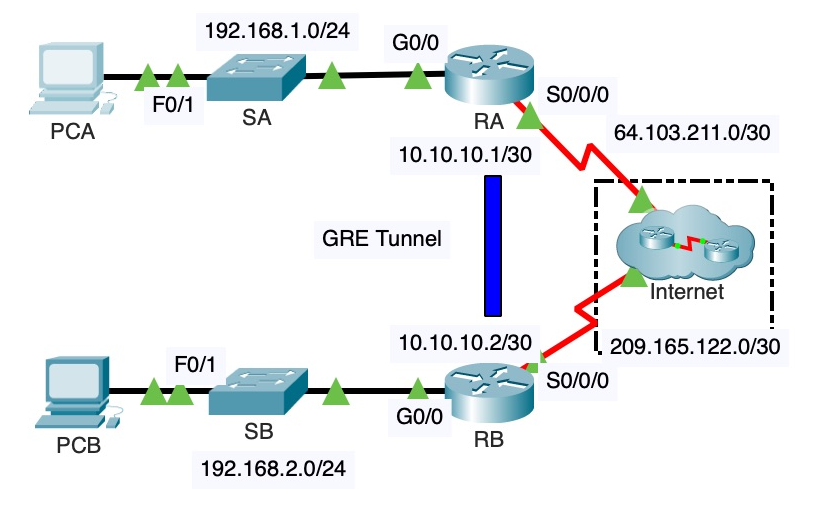
\includegraphics[width=0.95\linewidth]{images/topology.png}
\caption{Топология на задачата с двете LAN мрежи и предвидения GRE тунел.}
\end{figure}
\section{Начални проверки}
Началната оценка на PT Activity е 0/100. На RA командата \texttt{show ip interface brief} показва G0/0 с адрес 192.168.1.1 и S0/0/0 с адрес 64.103.211.2 в състояние up/up. Налице е предварително зададен маршрут по подразбиране през S0/0/0.

Преди конфигурирането на RB е изпълнен \texttt{ping 64.103.211.2} от RB към публичния интерфейс на RA: 5/5 успешни отговора, RTT 19/25/30 ms. Това потвърждава свързаността през транзитната мрежа. В този момент RA вече е конфигуриран, но тунелът и маршрутът в RB още липсват. Ping от PCB към PCA тогава е неуспешен: 0/4 отговора.

\section{Конфигуриране на тунела}
На всеки маршрутизатор е създаден Tunnel0 с адрес от 10.10.10.0/30. Източникът е локалният сериен интерфейс S0/0/0, а крайната точка е публичният адрес на отсрещния маршрутизатор. Зададени са режим GRE/IP и \texttt{no shutdown}. Статичният маршрут към отдалечената LAN използва адреса на отсрещния Tunnel0 като следващ скок.
\Needspace{14\baselineskip}
\subsection{Команди на RA}
\lstinputlisting{configs/RA.commands}
\Needspace{14\baselineskip}
\subsection{Команди на RB}
\lstinputlisting{configs/RB.commands}
Конфигурациите са записани с \texttt{write memory}; и двата маршрутизатора връщат \texttt{[OK]}. Предварително зададените LAN и WAN адреси са запазени.

\section{Проверки след конфигурирането}
На RA \texttt{show interfaces tunnel 0} показва Tunnel0 up/up, адрес 10.10.10.1/30, източник 64.103.211.2, крайна точка 209.165.122.2 и \texttt{Tunnel protocol/transport GRE/IP}. На RB \texttt{show ip interface brief} също показва Tunnel0 up/up, с адрес 10.10.10.2.

В маршрутната таблица на RB се появяват директно свързаната мрежа 10.10.10.0/30 през Tunnel0 и статичният маршрут 192.168.1.0/24 през 10.10.10.1. Ping от RB към 10.10.10.1 завършва с 5/5 отговора и RTT 24/27/35 ms.
\begin{figure}[H]
\centering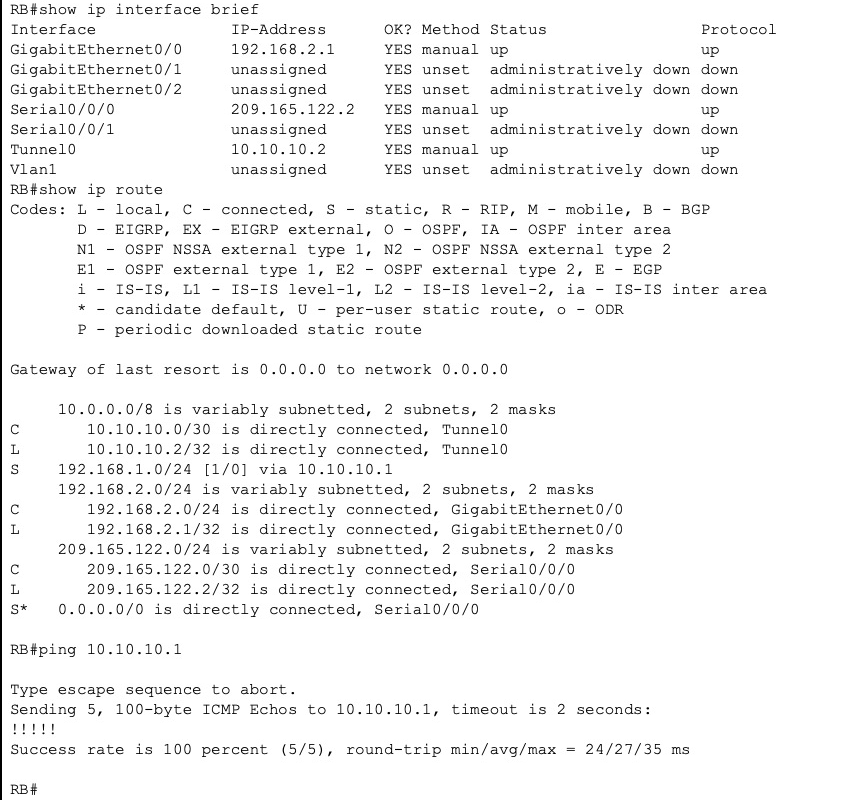
\includegraphics[width=0.95\linewidth]{images/rb-routing.png}
\caption{Състояние на интерфейсите, маршрутна таблица на RB и успешен ping през тунела.}
\end{figure}

\subsection{Свързаност между крайните устройства}
Първият ping от PCB към 192.168.1.2 след завършването на тунела е с 3/4 отговора и RTT 20/28/36 ms. Повторният тест е с 4/4 отговора, без загуби, RTT 27/29/33 ms и TTL 126. Полезният товар е 32 bytes. Времената са измерени в Packet Tracer и не описват производителността на физическа мрежа.
\begin{figure}[H]
\centering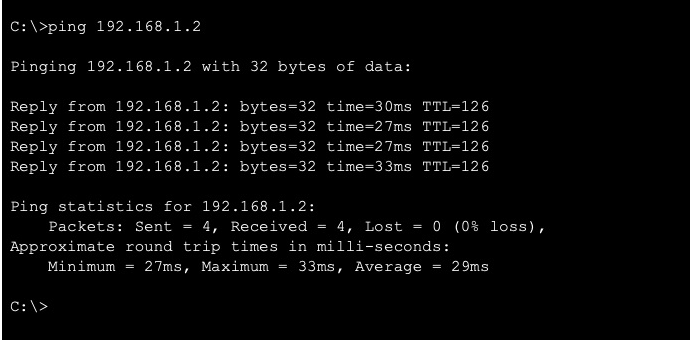
\includegraphics[width=0.9\linewidth]{images/pcb-ping.png}
\caption{Повторен успешен ping от PCB към PCA -- 4/4 отговора.}
\end{figure}



\subsection{Проследяване на пътя от PCA към PCB}
Командата \texttt{tracert 192.168.2.2} завършва успешно за три стъпки:
\begin{lstlisting}
1   0 ms    0 ms    0 ms    192.168.1.1
2  26 ms   11 ms   27 ms    10.10.10.2
3  31 ms   25 ms   26 ms    192.168.2.2
Trace complete.
\end{lstlisting}
В изхода се виждат LAN адресът на RA, тунелният адрес на RB и адресът на PCB. Публичните адреси на транзитната мрежа не се показват като отделни стъпки.
\begin{figure}[H]
\centering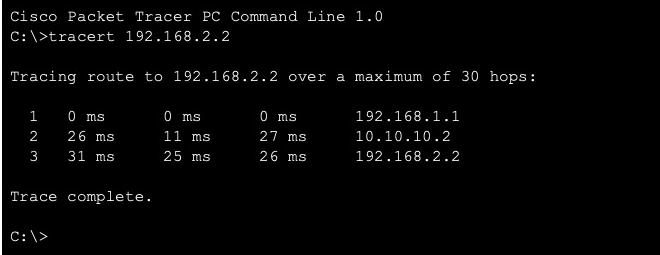
\includegraphics[width=0.95\linewidth]{images/pca-trace.png}
\caption{Проследяване от PCA към PCB през GRE тунела.}
\end{figure}

\Needspace{12\baselineskip}
\subsection{Автоматично оценяване}
PT Activity отчита \textbf{100/100 точки}. В Assessment Items са изпълнени 12/12 елемента: 10/10 за GRE конфигурациите, оценени с 90/90 точки, и 2/2 за IPv4 статичните маршрути, оценени с 10/10 точки.
\begin{figure}[H]
\centering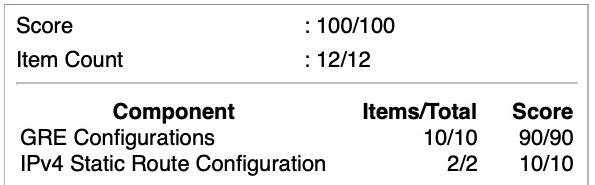
\includegraphics[width=0.95\linewidth]{images/score.png}
\caption{Оценка 100/100 за GRE тунела и статичната маршрутизация.}
\end{figure}


\clearpage
\section{Диагностика и отстраняване на грешки в GRE}
\subsection{Постановка и адресен план}
Задачата „Packet Tracer -- Troubleshooting GRE“ изисква откриване и поправяне на грешки в предварително създадена мрежа, последвано от ping от PCB към PCA и проследяване на обратния път. Началната оценка е 0/100. Адресите са независими от тези в първата задача.

\begin{table}[H]
\centering\small
\caption{Правилен адресен план за Troubleshooting GRE}
\begin{tabular}{llll}
\toprule Устройство & Интерфейс & IPv4 адрес & Маска \\\midrule
RA & G0/0 & 172.31.0.1 & /24 \\
RA & S0/0/0 & 209.165.122.2 & /30 \\
RA & Tunnel0 & 192.168.1.1 & /30 \\
RB & G0/0 & 172.31.1.1 & /24 \\
RB & S0/0/0 & 64.103.211.2 & /30 \\
RB & Tunnel0 & 192.168.1.2 & /30 \\
PCA & NIC & 172.31.0.2 & /24 \\
PCB & NIC & 172.31.1.2 & /24 \\\bottomrule
\end{tabular}
\end{table}
Шлюзовете на PCA и PCB са съответно 172.31.0.1 и 172.31.1.1. В адресната таблица на условието крайният хост е означен като PC-C, а в топологията и стъпките за проверка -- като PCB.
\begin{figure}[H]
\centering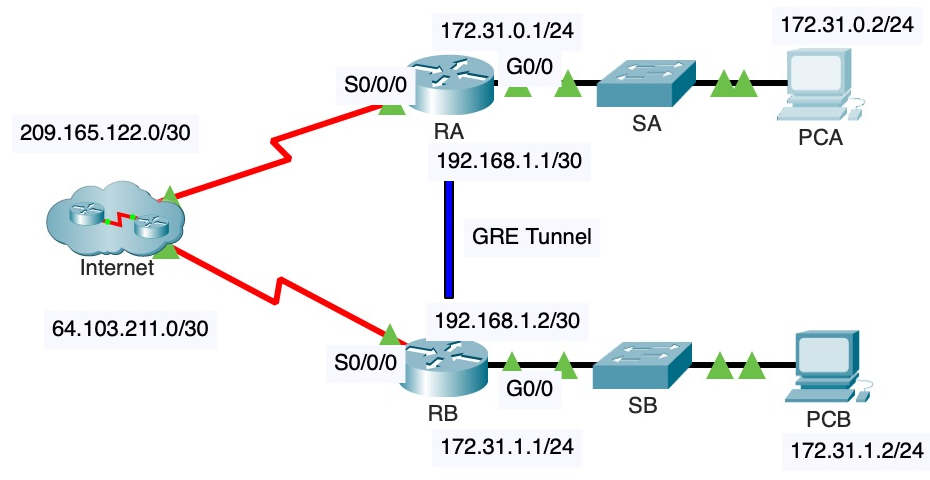
\includegraphics[width=0.95\linewidth]{images/troubleshooting-topology.png}
\caption{Топология и адреси на задачата за диагностика.}
\end{figure}

\subsection{Открити грешки и корекции}
Командата \texttt{show running-config} на двата маршрутизатора разкрива следните несъответствия:
\begin{enumerate}
\item RA, Tunnel0: зададен е LAN адресът 172.31.0.1/24. Заменен е с 192.168.1.1/30.
\item RA, G0/0: зададен е тунелният адрес 192.168.1.1/30. Възстановени са 172.31.0.1 и маска 255.255.255.0.
\item RA, маршрут към 172.31.1.0/24: следващият скок е публичният адрес 64.103.211.2. Маршрутът е заменен с такъв през тунелния адрес 192.168.1.2.
\item RB, източник на Tunnel0: зададен е G0/0. Заменен е със Serial0/0/0, който носи публичния адрес 64.103.211.2.
\item RB, крайна точка на Tunnel0: зададен е тунелният адрес 192.168.1.1. Заменен е с публичния адрес на RA -- 209.165.122.2.
\end{enumerate}
Преди корекциите ping от RB към публичния адрес 209.165.122.2 е успешен: 5/5 отговора и RTT 19/25/30 ms. Следователно транзитната свързаност е налична. Правилно зададените адреси на RB, неговият маршрут към 172.31.0.0/24 през 192.168.1.1 и маршрутите по подразбиране са запазени.

\Needspace{18\baselineskip}
\subsection{Приложени команди}
Първо са поправени крайните точки на RB, след което адресите и маршрутът на RA. За да няма припокриване при размяната на адресите на RA, първо е премахнат грешният адрес на Tunnel0.
\textbf{RA:}
\lstinputlisting{configs/RA-troubleshooting.commands}
\Needspace{9\baselineskip}
\textbf{RB:}
\lstinputlisting{configs/RB-troubleshooting.commands}
И двете конфигурации са записани с \texttt{write memory}, с потвърждение \texttt{[OK]}.

\subsection{Проверка на тунела и маршрутизацията}
На RA интерфейсите G0/0, S0/0/0 и Tunnel0 са up/up с правилните адреси. Маршрутната таблица съдържа 172.31.1.0/24 през 192.168.1.2 и директно свързаната тунелна мрежа 192.168.1.0/30. Ping от RA към 192.168.1.2 е успешен: 5/5 отговора, RTT 15/21/27 ms.
\begin{figure}[H]
\centering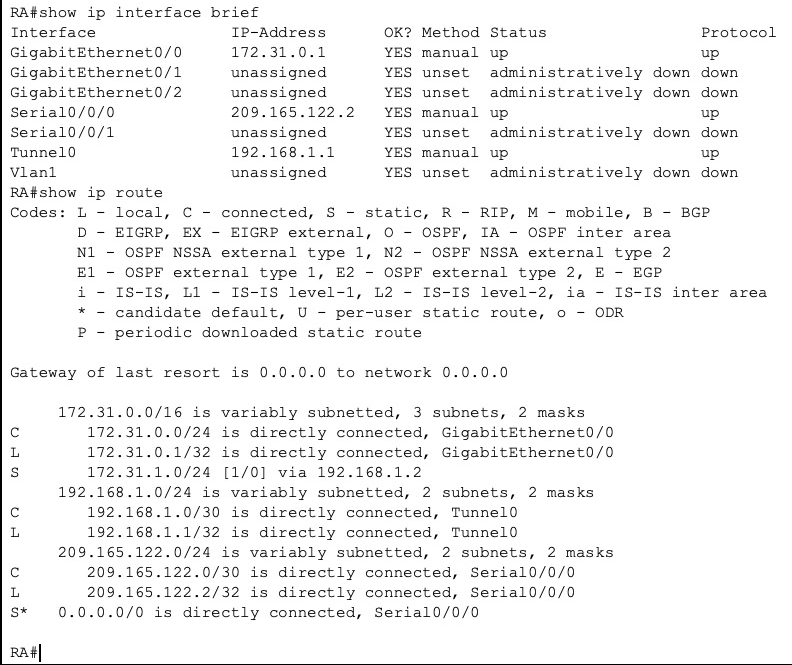
\includegraphics[width=0.9\linewidth]{images/troubleshooting-routing.png}
\caption{Поправените адреси и статичният маршрут на RA.}
\end{figure}

\subsection{Крайни проверки и оценяване}
Първият ping от PCB към PCA след поправките има 3/4 отговора и RTT 21/25/30 ms. Повторният тест към 172.31.0.2 завършва с \textbf{4/4 отговора и 0\% загуби}, RTT 22/28/33 ms и TTL 126 при 32 bytes полезен товар.
\begin{figure}[H]
\centering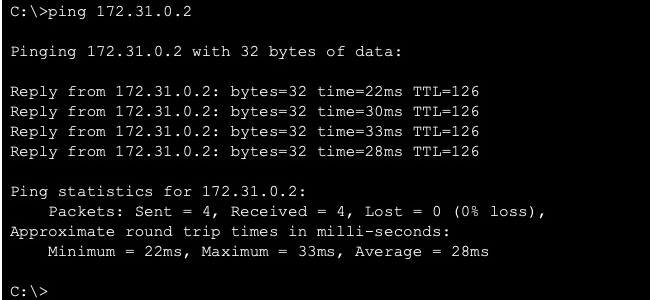
\includegraphics[width=0.9\linewidth]{images/troubleshooting-ping.png}
\caption{Повторен ping от PCB към PCA след отстраняване на грешките.}
\end{figure}
Командата \texttt{tracert 172.31.1.2} от PCA завършва успешно:
\begin{lstlisting}
1   0 ms    0 ms    0 ms    172.31.0.1
2  23 ms   19 ms   20 ms    192.168.1.2
3  15 ms   18 ms   20 ms    172.31.1.2
Trace complete.
\end{lstlisting}
Виждат се LAN адресът на RA, тунелният адрес на RB и PCB. Публичните транзитни адреси не се появяват като отделни стъпки.
\begin{figure}[H]
\centering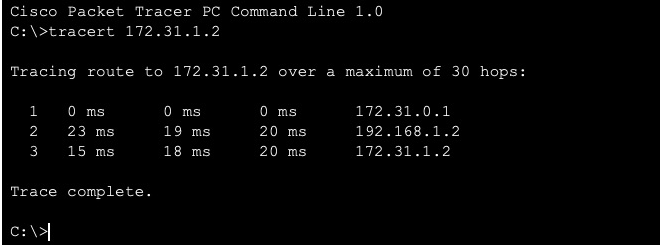
\includegraphics[width=0.95\linewidth]{images/troubleshooting-trace.png}
\caption{Успешно проследяване от PCA към PCB през поправения тунел.}
\end{figure}
\Needspace{10\baselineskip}
Автоматичната проверка отчита \textbf{100/100 точки и 5/5 правилни елемента}: адрес на Tunnel0 на RA, адрес и маска на G0/0 на RA, статичен маршрут на RA и крайна точка на тунела на RB. Всеки елемент носи 20 точки. Източникът на тунела на RB също е поправен, въпреки че не е отделен оценяван елемент.
\begin{figure}[H]
\centering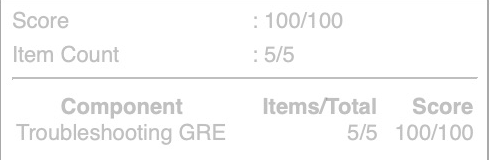
\includegraphics[width=0.9\linewidth]{images/troubleshooting-score.png}
\caption{Крайна оценка за Troubleshooting GRE -- 100/100, 5/5 елемента.}
\end{figure}

\section{Заключение}
Създаден е работещ GRE тунел между RA и RB. Двете частни мрежи обменят трафик чрез статични маршрути към тунелните адреси. Крайният ping от PCB към PCA е без загуби, а traceroute от PCA към PCB показва три стъпки, без публичните транзитни адреси. Автоматичната проверка потвърждава изпълнението с 100/100 точки.

Във втората задача са отстранени грешки в адресирането, статичната маршрутизация и крайните точки на GRE. Повторният ping е без загуби, а traceroute потвърждава преминаването през тунела. И двете задачи са оценени със 100/100 точки.

В папката \texttt{cisco/} са записани завършените файлове \texttt{Configuring GRE.pka} и \texttt{Troubleshooting GRE.pka}. Папките \texttt{configs/}, \texttt{evidence/} и \texttt{images/} съдържат приложените команди, текстов препис на резултатите и екранните снимки. Командните файлове съдържат направените настройки, а не пълни running-config конфигурации.

\begin{thebibliography}{9}
\bibitem{activity} Cisco Networking Academy. Packet Tracer -- Configuring GRE. Условия, адресна таблица и вградено оценяване в приложения PKA файл. Изпълнение на 09.11.2026 г.
\bibitem{troubleshooting} Cisco Networking Academy. Packet Tracer -- Troubleshooting GRE. Условия, адресна таблица и вградено оценяване в приложения PKA файл. Изпълнение на 18.11.2026 г.
\end{thebibliography}
\end{document}
